\documentclass[a4paper,11pt,twocolumn]{article}

% Common lightweight packages
\usepackage[paperwidth=210mm,paperheight=297mm,margin=8pt]{geometry} % A4, no margins
\usepackage{ZFPredef}

\begin{document}
\textbf{\huge HF}
\raggedright

\newcommand{\cp}{
\begin{tikzpicture}\node[circle, inner sep = 1pt,draw] {+};\end{tikzpicture}\hspace{5pt}}
\newcommand{\cm}{
\begin{tikzpicture}\node[circle, inner sep = 3pt,draw] {-};\end{tikzpicture}\hspace{5pt}}
\newcommand{\fb}{\textcolor{red}{Fehlt Bild}}

\newcommand{\ggt}[2]{%
  {\mathbin{\genfrac{}{}{-10pt}{3}{\color{black}#1}{\color{orange}#2}}}%
}




%\section{Grundlagen}


\Term{Mikrostreifenleitungen}:
Quasi-TEM-Wellen
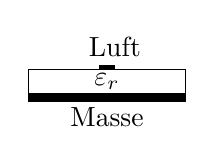
\begin{tikzpicture}
    \draw (0,0) rectangle (2,0.3) node[midway] {$\varepsilon_r$};
    \filldraw (0,0) rectangle (2,-0.1) node[midway, below] {Masse};
    \filldraw (0.9,0.3) rectangle (1.1,0.35) node[at end, above] {Luft};
\end{tikzpicture}

\Term{Triplate Leitung}:
TEM-Wellen

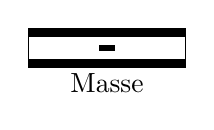
\begin{tikzpicture}
    \draw (0,0) rectangle (2,0.3);
    \filldraw (0,0) rectangle (2,-0.1) node[midway, below] {Masse};
    \filldraw (0,0.3) rectangle (2,0.4);
    \filldraw (0.9,0.12) rectangle (1.1,0.18);
\end{tikzpicture}




\Term{Leitungsgleichung}
$\gamma, Z_L$

$U = U_f \e^{- \gamma z} + U_b \e^{\gamma z}$
$I = \frac{U_f}{Z_L} \e^{-\gamma z} - \frac{U_f}{Z_L} \e^{\gamma z}$

Normierungs:

$u = \frac{U}{\sqrt{Z_L}}$ , $i = I \sqrt{Z_0}$ , $U_f = I_f Z_L$

$u = u_f\e^{-\gamma z} + u_b\e^{\gamma z} = a + b$\\
$i = a-b$


\Term{Matrixbeschreibungen}
\begin{pitemize}
    \item \Term{S-Parameter (Streuparameter)}:
    \begin{pitemize}
        \item Beschreibung über Wellen ($a_i$ (Eingang Oben), $b_i$ (Ausgang unter), Nummer sind die Seite)
        \item $\begin{pmatrix} b_1 \\ b_2 \end{pmatrix}
                =
                \begin{pmatrix} S_{11} & S_{12} \\ S_{21} & S_{22} \end{pmatrix}
                \begin{pmatrix} a_1 \\ a_2 \end{pmatrix}$
            \begin{pitemize}
                \item $S_{11} \big|_{a_2 = 0} = \frac{b_1}{a_1}$: Reflexion Eingang
                \item $S_{21} \big|_{a_2 = 0} = \frac{b_2}{a_1}$: Transmission (Verstärkung)
                \item $S_{12}$: Rückwirkung
                \item $S_{22}$: Reflexion Ausgang
            \end{pitemize}
    \end{pitemize}

    \item \Term{Impedanzparameter}:
    \begin{pitemize}
        \item $U_1 = Z_{11}I_1 + Z_{12}I_2$
        \item $U_2 = Z_{21}I_2 + Z_{22}I_2$
    \end{pitemize}

    \item \Term{T-Parameter (ABCD-Parameter)}:
    \begin{pitemize}
        \item Zusammenhang von Spannungen und Strömen
        \item Ideal für Kaskadierung (Matrizenmultiplikation)
        \item $\begin{pmatrix} U_1 \\ I_1 \end{pmatrix}
            =
            \begin{pmatrix} A & B \\ C & D \end{pmatrix}
            \begin{pmatrix} U_2 \\ -I_2 \end{pmatrix}$
    \end{pitemize}


    \item \Term{Kettenparameter}:
    \begin{pitemize}
        \item Alternative Darstellung der ABCD-Parameter
        \item $\begin{pmatrix} U_1 \\ I_1 \end{pmatrix}
            =
            \begin{pmatrix} A & B \\ C & D \end{pmatrix}
            \begin{pmatrix} U_2 \\ I_2 \end{pmatrix}$
    \end{pitemize}
\end{pitemize}

%
\section{Koppler}
\renewcommand{\ort}{topics/Koppler}

\Term{Taktanregung}
\begin{pitemize}
    \item \Term{Gleichtaktanregung}: \cp
Signale gleicher Amplitude und gleicher Phase.
\begin{pitemize}
    \item $Z_e$
    \item $a_1^+ = \frac{1}{2} a_1,a_4^+ = \frac{1}{2} a_1$
\end{pitemize}
    \item \Term{Gegentaktanregung}: \cm
Signale gleicher Amplitude und engegengesetzer Phase.
\begin{pitemize}
    \item $Z_d$
    \item $a_1^- = \frac{1}{2} a_1,a_4^- = -\frac{1}{2} a_1$
\end{pitemize}
    \item Überlagerung: $a_1^+  + a_1^- = a_1$ , $a_4^+  + a_4^- = 0$
\end{pitemize}


\subsection{Leitungskoppler}

\bild{topics/Koppler/Leitungskoppler}

\bild{topics/Koppler/Bsp Leitungskoppler}

$|\Gamma|^2 = \frac{P2}{P1} \left\lvert\frac{S_{41}}{S_{32}S_{21}}\right\rvert^2$

\Term{Zweifach Symmetrischer Zweitor}:

\bild{topics/Koppler/Leitungskoppler 2}

Allseit. Anpassung: \\$S_{11}=S_{22}=S_{33}=S_{44}=0$\\
Symmetrien und Reziprok:\\
$S_{41}=S_{14}=S_{32}=S_{23}$\\
$S_{12}=S_{21}=S_{34}=S_{43}$\\

\Term{Mit Gleich- und Gegentaktanregung}:\\
$b_1= b_1^+ + b_1^- = S_{11}^+ a_1^+ + S_{11}^- a_1^- = \frac{1}{2} (S_{11}^+ + S_{11}^-) a_1$, $\rightarrow S_{11}$
$b_2= b_2^+ + b_2^- = S_{21}^+ a_1^+ + S_{21}^- a_1^- = \frac{1}{2} (S_{21}^+ + S_{21}^-) a_1$, $\rightarrow S_{21}$
$b_3= b_2^+ + b_2^- = S_{21}^+ a_4^+ + S_{21}^- a_4^- = \frac{1}{2} (S_{21}^+ - S_{21}^-) a_1$, $\rightarrow S_{31}$
$b_4= b_4^+ + b_4^- = S_{11}^+ a_4^+ + S_{11}^- a_4^- = \frac{1}{2} (S_{11}^+ - S_{11}^-) a_1$, $\rightarrow S_{41}$




\Term{Normierung der Widerstände}:
$z_e = \frac{Z_e}{Z_0}$,$z_d = \frac{Z_d}{Z_0}$ \\
$\begin{bmatrix}
    A^\ggt{+}{-} & B^\ggt{+}{-} \\ C^{\ggt{+}{-}} & D^{\ggt{+}{-}}
\end{bmatrix} = \begin{bmatrix}
    \cos(\beta l) & jz_{\ggt{e}{d}}\sin(\beta l) \\
    j\frac{1}{z_{\ggt{e}{d}}}\sin(\beta l) & \cos(\beta l)
\end{bmatrix}$

$S_{11}^+ = \frac{A^+ + B^+ - C^+ - D^+}{A^+ + B^+ + C^+ + D^+} = \frac{jz_e\sin(\beta l) -
    j\frac{1}{z_e}\sin(\beta l) }{2\cos(\beta l) + j(z_e + \frac{1}{z_e}) \sin(\beta l)}$\\

$S_{11}^- = \frac{j(z_d - \frac{1}{z_d})\sin(\beta l) }{2\cos(\beta l) + j(z_d + \frac{1}{z_d}) \sin(\beta l)}$
$S_{21}^+ = \frac{2}{A^+ + B^+ + C^+ + D^+} = \frac{2}{2\cos(\beta l) + j(z_e + \frac{1}{z_e}) \sin(\beta l)}$\\
$S_{21}^+ = \frac{2}{A^- + B^- + C^- + D^-} = \frac{2}{2\cos(\beta l) + j(z_d + \frac{1}{z_d}) \sin(\beta l)}$

Allseitige anpassung $S_{11} = 0 \rightarrow S_{11}^+ = - S_{11}^- \rightarrow z_e = \frac{1}{z_d} \leftrightarrow z_ez_d = 1 \rightarrow Z_eZ_d = Z_0^2$
Entkoppelte Tore: $S_{31} = \frac{1}{2}(S_{21}^+ - S_{21}^-) = 0 \rightarrow S_{21}^+ = S_{21}^-$
$S_{21} = S_{21}^+ = \frac{2}{2\cos(\beta l) + j(z_e + \frac{1}{z_e}) \sin(\beta l)}$\\
$S_{41} = \frac{1}{2}(S_{11}^+ - S_{11}^-) = S_{11}^+ = \frac{j(z_e - \frac{1}{z_e})\sin(\beta l) }{2\cos(\beta l) + j(z_e + \frac{1}{z_e}) \sin(\beta l)}$

$\angle(S_{21}, S_{41}) = 90^\circ$\\
Mehrstufig wenn höhere Breitband.

\subsection{Ringkoppler}

\bild{topics/Koppler/Ringkoppler}

\begin{pitemize}
    \item 3dB-Kopplung: 1 $\rightarrow$ 2 und 1 $\rightarrow$ 3
    \item Entkopplung: 1 und 4
    \item Einspeisung an 1
    \item $Z_1 = ?$, $Z_2 = ?$ 
\end{pitemize}


\begin{pitemize}
    \item \Term{Gleichtakt}
    \begin{pitemize}
        \item \cp  an 1 und 4: $a_1^+ = \frac{1}{2}a_1, a_4^+ = \frac{1}{2}a_1$ 
        \item \bild{topics/Koppler/Ringkoppler Gleichtakt}
    \end{pitemize}
    \item \Term{Gegentakt}
    \begin{pitemize}
        \item \cm  an 1 und 4: $a_1^- = \frac{1}{2}a_1, a_4^- = -\frac{1}{2}a_1$
        \item \bild{topics/Koppler/Ringkoppler Gegentakt}
    \end{pitemize}
\end{pitemize}


\bild{topics/Koppler/Leitungsdarstellung}
\begin{pitemize}
    \item $Z_{ein} = Z_L \frac{Z_A + jZ_L \tan(\beta l)}{Z_L + jZ_A \tan(\beta l)}$
    \item $\tan(\beta l) = \tan(\frac{2\pi}{\lambda} \frac{\lambda}{8}) = \tan(\frac{\pi}{4}) = 1$
    \item \cp $Z_A \rightarrow \infty \Rightarrow Z_{ein,LL}^+ = \lim_{Z_A \rightarrow \infty}\limits Z_{ein} = -jZ_L = -jZ_1$
    \item \cm $Z_A \rightarrow 0 \Rightarrow Z_{ein,LL}^- = jZ_L = jZ_1 = j\frac{1}{Y_1}$
\end{pitemize}

Kettenmatrizen fortsetzung

$\left[M^\ggt{+}{-}\right] = \begin{bmatrix}
    1 & 0 \\ -jY_1Z_0 & 1
\end{bmatrix}\begin{bmatrix}
    0 & j\frac{Z_2}{Z_0} \\ j\frac{Z_0}{Z_2} & 0
\end{bmatrix}\begin{bmatrix}
    1 & 0 \\ -jY_1Z_0 & 1
\end{bmatrix}
= \begin{bmatrix}
    \ggt{+}{-}Z_2Y_1 & j \frac{Z_2}{Z_0}\\ j\frac{Z_0}{Z_2} - jY_1^2Z_0Z_2 & \ggt{+}{-}Y_1Z_2
\end{bmatrix} = \begin{bmatrix}
    A^\ggt{+}{-} & B^\ggt{+}{-} \\ C^\ggt{+}{-} & D^\ggt{+}{-}
\end{bmatrix}$

Anforderung: Allseitige Anpassung
\begin{pitemize}
    \item $S_{11} = \frac{1}{2}(S_{11}^+ + S_{11}^-) \overset{!}{=} 0$
    \item $S_{41} = S_{14} = \frac{1}{2}(S_{11}^+ - S_{11}^-) \overset{!}{=} 0$
    \item $S_{11}^+ = \frac{A^+ + B^+ - C^+ - D^+}{A^+ + B^+ + C^+ + D^+} \overset{!}{=} 0$
    \item Da $A^+ = D^+ \Rightarrow B^+ = C^+$
    \item $\frac{Z_2}{Z_0} = \frac{Z_0}{Z_2} - Y_1^2 Z_2 Z_0$
    \item $|S_{21}| = \lvert\frac{1}{2} \left(S_{21}^+ + S_{21}^-\right)\rvert = |S_{31}| = \lvert\frac{1}{2} \left(S_{21}^+ - S_{21}^-\right)\rvert$
    \item $\frac{Z_2}{Z_0} = Y_1 Z_2 \Rightarrow Y_1 = \frac{1}{Z_0}$
    \item $1 = \frac{Z_0^2}{Z_2^2} - Y_1^2Z_0^2 \Rightarrow Z_2 = \frac{1}{\sqrt{2}}Z_0$
\end{pitemize}

\begin{pitemize}
    \item $\angle(S_{21}, S_{31}) = 90^\circ$
    \item 3dB-Kopplung: 1 $\rightarrow$ 2 und 1 $\rightarrow$ 3
    \item Entkopplung: 1 und 4
\end{pitemize}


\subsubsection{Rat-Race-Koppler}
\bild{topics/Koppler/Rat-Race-Koppler}
\begin{pitemize}
    \item Einsp. 1: 3 entkoppelt, $\angle(S_{21}, S_{41}) = 0^\circ$
    \item Einsp. 3: 1 entkoppelt, $\angle(S_{23}, S_{43}) = 180^\circ$
\end{pitemize}








\subsection{Resistiver Koppler}
\bild{topics/Koppler/ResKop}

Synthese: All. Anpassung
\begin{pitemize}
    \item $S_{31} = S_{13} = S_{24} = S_{42} = 0$
\end{pitemize}
$S_{11} = \frac{Z_{ein} -Z_0}{Z_{ein} + Z_0}$

\cp und \cm an 1 und 4.\\

\bildf{r\_koppler}

\cp $\Rightarrow$ in der Symmetrieeben $\Rightarrow$ LL
\begin{pitemize}
    \item \bildf{r\_koppler\_plus}
    \item $S_{11}^+ = \frac{2R_2 + Z_0 - Z_0}{2 R_2 + Z_0 + Z_0} = \frac{R_2}{R_2+Z_0}$
\end{pitemize}

\cm
\begin{pitemize}
    \item \bildf{r\_koppler\_minus}
    \item $S_{11}^- = -\frac{Z_0}{R_1 + Z_0}$
\end{pitemize}

$S_{11} = \frac{1}{2}(S_{11}^+ + S_{11}^-) \overset{!}{=} 0 \Rightarrow S_{11}^+ = -S_{11}^-$ \\
$\frac{R_2}{R_2 + Z_0} = \frac{Z_0}{R_1 + Z_0} \Rightarrow R_1R_2 = Z_0^2$

$S_{41} = \frac{1}{2}(S_{11}^--S_{11}^-) = S_{11}^+ = \frac{R_2}{R_2 + Z_0}$\\
$S_{21} = \frac{Z_0}{Z_0 + R_2}$


Häufige Wahl: $R_1 = R_2 = Z_0 \Rightarrow S_{21}=S_{41} = \frac{1}{2}$

Nullgradkoppler: $\angle(S_{21}, S_{41}) = 0^\circ$

\subsection{Transformatorkoppler}

\bildf{trafo\_koppler}

\begin{pitemize}
    \item Transformator sei ideal
    \item aus Symmetrie sind 1 und 4 entkoppelt
    \item bei Einspeisung an 1 $\Rightarrow$ Signale an 2 und 3 in Gegenphase
    \item bei Einspeisung an 4 $\Rightarrow$ Signale an 2 und 3 in Phase
    \item $\Rightarrow$ Signale an 2 und 3 entkoppelt mit $Z = \frac{Z_0}{2}$
\end{pitemize}


\subsection{Nullgradkoppler/Signalteiler}

\bildf{NullGradKoppler}
\bildf{null\_grad\_koppler\_EB}
\begin{pitemize}
    \item \cp und \cm and 2 und 3
    \item \cp an 2 und 3:
    \begin{pitemize}
        \item \bildf{null\_grad\_koppler\_plus}
        \item $Z_{ein} \frac{Z_1}{2Z_0} \overset{!}{=} 0 \Rightarrow Z_1 = \sqrt{2}Z_0$
    \end{pitemize}
    \item \cm an 2 und 3:
    \begin{pitemize}
        \item \bildf{null\_grad\_koppler\_minus}
        \item $\frac{R}{2}=Z_0 \Rightarrow R = 2Z_0$
    \end{pitemize}
\end{pitemize}
%\section{Messung}
\renewcommand{\ort}{topics/Messung}


\subsection{Breitbanddetektoren}

\bildf{BBDet}
Nicht Lineare Effekte(Verständnis)
\bildf{BBDetErg}


\subsection{Skalare Zweitormessung}

\subsubsection{Substitionsverfahren}
\bildf{skalar\_zt\_substitution}
$P_2 = \lvert S_{21}\rvert^2 P_g \Leftrightarrow  \lvert S_{21}\rvert^2 = \frac{P_2}{P_1}$

\subsubsection{Leitungskoppler}
\bildf{skalar\_zt\_1}
$P_1 = K P_g$\\
$\lvert S_{21}\rvert^2 = \frac{K}{(1 - K)}\frac{P_2}{P_1}$

\bildf{skalar\_zt\_2}

\begin{pitemize}
    \item $P_2 = \lvert S_{21}\rvert^2 (1-k)^2 P_g$
    \item $P_1 = k P_g$
    \item $P_3 = \lvert S_{11}\rvert^2 (1-k)^2 k P_g$
    \item $\lvert S_{21}\rvert^2 = \frac{P_2}{P_1}\frac{k}{(1-k)^2}$
    \item $\lvert S_{11}\rvert^2 = \frac{P_3}{P_1}\frac{1}{(1-k)^2}$
\end{pitemize}


\subsubsection{}

\bildf{skalar\_zt\_3}
\begin{pitemize}
    \item $P_1 = k P_g$
    \item $P_2 = \lvert S_{21}\rvert^2 (1-2k) P_g$
    \item $P_3 = k \lvert S_{11}\rvert^2 (1-2k) P_g$
    \item $\lvert S_{21}\rvert^2 = \frac{P_2}{P_1} \frac{k}{1-2k}$
    \item $\lvert S_{11}\rvert^2 = \frac{P_3}{P_1} \frac{1}{1-2k}$
\end{pitemize}



\subsubsection{Fehler bei Transmissionmessung}

Annahme: Fehlanpassung am Generator und am Leistungsdetektor
$\rightarrow$ Fehlermodell
\bildf{transmission\_error}

\begin{pitemize}
    \item $P_{Det} = \lvert b_2\rvert^2$
    \item Ohne MO:
    \begin{pitemize}
        \item \bildf{error\_ohne\_MO}
        \item $P_{g_{ver}} = \abs{a_1}^2$
        \item $b_2 = V_{21}a_1$
        \item $P_{Det} = \abs{b_1}^2 = \abs{V_{21}}^2 \abs{a_1}^2$
        \item $R_{22} = \Gamma_g$
        \item $T_{11} = \Gamma_L$
        \item Zu Transmissionmatrizen
        \item $\left[\Sigma_V\right] = \left[\Sigma_R\right] \left[\Sigma_T\right] = \frac{1}{R_21}\begin{bmatrix}
            -\Delta_R & R_{11} \\ -R_{22} & 1
        \end{bmatrix}\frac{1}{T_21}\begin{bmatrix}
            -\Delta_T & T_{11} \\ -T_{22} & 1
        \end{bmatrix}$
        \item $V_{21} = \frac{1}{\Sigma_{V_{22}}} = \frac{R_21 T_21}{1 - R_22 T_11}$
        \item $P_{Det} = \abs{\frac{R_{21} T_{21}}{1 - R_{22} T_{11}}}^2 P_{g_{ver}}$
        \item Annahme: Fehlerzweitoren verlustlos: 
        \begin{pitemize}
            \item $\abs{R_{21}}^2 = \abs{R_{12}}^2 = 1 - \abs{R_22}^2$
            \item $ \abs{T_{21}}^2 = 1 - \abs{T_11}^2$
        \end{pitemize}
        \item $P_{Det} = \frac{(1 - \abs{\Gamma_g}^2)(1 - \abs{\Gamma_L}^2)}{\abs{1 - \Gamma_g \Gamma_L}^2} P_{g_{ver}}$    
    \end{pitemize}
    \item Mit MO:
    \begin{pitemize}
        \item \bildf{error\_mit\_MO}
        \item $W_{21} = \frac{1}{\Sigma_{W_{22}}}$
        \item $\Sigma_W = \frac{1}{R_{21}S_{21}T_{21}} \begin{bmatrix}-\Delta_R & R_{11} \\ -R_{22} & 1\end{bmatrix}\begin{bmatrix}-\Delta_S & S_{11} \\ -S_{22} & 1\end{bmatrix}\begin{bmatrix}-\Delta_T & T_{11} \\ -T_{22} & 1\end{bmatrix}$
        \item $W_{21} = \frac{R_{21}S_{21}T_{21}}{1 - R_{22}S_{11} - S_{22}T_{11} + T_{11}R_{22}\Delta_S}$
        \item $\abs{\hat{S}_{21}}^2 = \frac{\abs{W_{21}}^2}{\abs{V_{21}}^2} = \abs{S_{21}}^2 \frac{\abs{1 - \Gamma_g \Gamma_L}^2}{\abs{(1- \Gamma_g S_11)(1- \Gamma_L S_22) - S_{12}S_{21} \Gamma_g \Gamma_L}^2}$
    \end{pitemize}
    \item Beispiel für Fehlerschätzung:
    \begin{pitemize}
        \item MO: $\abs{S_{12}} = \abs{S_{21}} = \frac{1}{2}$ , $\abs{S_{11}} = \abs{S_{22}} = 0.1$
        \item Messsystem: $\abs{\Gamma_g} = 0.1$, $\abs{\Gamma_L} = 0.1$
        \item $\abs{\hat{S}_{21}}^2 = \frac{\abs{1 \pm 0.01}^2}{\abs{(1 \mp 0.01)^2 \mp 0.0025}^2} \abs{S_{21}}^2$
        \item $\abs{\hat{S}_{21}}^2 \approx \frac{1 \pm 0.02}{(1 \mp 0.02 \mp 0.0025)^2} \abs{S_{21}}^2$
        \item $\abs{\hat{S}_{21}}^2 \approx \frac{1 \pm 0.02}{1 \mp 0.045} \abs{S_{21}}^2 \approx (1 \pm 0.06) \abs{S_{21}}^2 \hat{=} 0.27 dB$
    \end{pitemize}
\end{pitemize}



\subsection{Vektorielle Netzwerkanalyse}

\bildfR{0.8}{vektor_netzwerkanalyse}

\begin{pitemize}
    \item Maß für fortlaufende Welle $f_{ZF, I}$
    \item Maß für reflektierte Welle $f_{ZF, II}$
    \item Maß für transmitierte Welle $f_{ZF, III}$
    \item \bildf{vna rampe}
\end{pitemize}
%\section{Messung}
\renewcommand{\ort}{topics/SPSchaltungen}


\subsection{Prototypfilter/Referenzfilter}

\fb \\
$Z_0 = 1 \Omega$
Normierung: bei $\omega_{ref} = \omega_c$:
\begin{pitemize}
    \item $\omega_c C = 2\Omega^{-1}$
    \item $\omega_c L = 1\Omega$
\end{pitemize}

\fb \\
$\abs{S_{21}(\omega_c)}^2 = \frac{1}{2}$


\subsection{Leitungsfilter}
für HF-Filter Übergang zu Leitungselementen

\fb\\

$Z_1 = Z_L \frac{Z_2 + jZ_L \tan(\beta l)}{Z_L + j Z_2\tan(\beta l)}$\\
$\beta l = \Theta = \frac{2\pi}{\lambda} l = \frac{2\pi}{\lambda} \frac{\lambda}{4} \frac{\omega}{\omega_0} = \frac{\pi}{2} \frac{\omega}{\omega_0}$

\fb Kurzschliessen von $Z_2$ \\

$Z_2 = 0 \Rightarrow Z_{1,KS} = jZ_L \tan(\beta l) \hat{=}$ induktiv
$Z_L \hat{=} \tilde{L}$ \\
\fb Leerlauf \\

$Z_2 \rightarrow \infty \Rightarrow Z_{1,LL} = Z_L \frac{1}{j\tan(\beta l)} \hat{=}$ kapazitiv
$Z_L \hat{=} \frac{1}{\tilde{C}}$ 

$\frac{w_c}{\omega_{ref} C} \Rightarrow \tilde{C} = C$\\

für $L = \tilde{L}$ und $C = \tilde{C}$:\\
\begin{equation}
\frac{\omega_{ref}}{\omega_c} = \tan(\beta l) = \tan(\frac{\pi}{2}\frac{\omega}{\omega_c})
\Leftrightarrow \omega = \omega_0 \frac{2}{\pi} \arctan(\frac{\omega_{ref}}{\omega_c})
\end{equation}

$\omega_{ref} \hat{=}$ Frequenz des Referenzfilter\\
$\omega$ ist die Frequenz des Leitungsfilters


\fb \\
\begin{pitemize}
\item $\omega_{ref} = 0 \Rightarrow \omega = 0$
\item $\omega_{ref} \rightarrow \infty \Rightarrow \omega = \omega_0 \frac{\pi}{2}\frac{2}{\pi} = \omega_0$
\item $\omega_{ref} = \omega_c \Rightarrow \omega = \omega_0 \frac{2}{\pi} \arctan(1) = \frac{\omega_0}{2}$
\end{pitemize}

2Draht-ESB:\\
\fb \\

Konzentrierte Elemente ersetzen durch Stichleitungen.
\begin{pitemize}
    \item Indiktivitäten: Am Ende KS Stichleitungen 
    \item \fb
    \item \fb
    \item Kapazitäten: Am Ende LL Stichleitungen
\end{pitemize}


\subsection{Butterworth-Hochpassfilter}
Prototypfilter:
\fb \fb\\


Übergang zum Leitungsfilter
\fb \fb\\

bei Mikrostreifenleitungen sind keine seriel liegenden Stichleitungen möglich.

\subsection{Kuroda Identitäten}

\fb \\

$S = j \tan{\beta L}$ Richardstransformation

$\frac{1}{\sqrt{1 - s^2}}\begin{bmatrix}
    1 & sL \\ 0 & 1
\end{bmatrix} \begin{bmatrix}
    1 & sZ_0 \\ \frac{s}{Z_0} & 1
\end{bmatrix} \overset{!}{=} \frac{1}{\sqrt{1 - s^2}}\begin{bmatrix}
    1 & sZ_1 \\ \frac{s}{Z_1} & 1
\end{bmatrix}\begin{bmatrix}
    1 & 0 \\ sC & 1
\end{bmatrix}$ \\

$\begin{bmatrix}
    q + s^2\frac{L}{Z_0} & s(L + Z_0) \\ \frac{s}{Z_0} & 1
\end{bmatrix} \overset{!}{=} \begin{bmatrix}
    1 + s^2Z_1C & sZ_1 \\ s(\frac{1}{Z_1} + C) & 1
\end{bmatrix} $

\begin{pitemize}
    \item $\frac{L}{Z_0} = Z_1 C$
    \item $Z_1 = L + Z_0$
    \item $\frac{1}{Z_0} = \frac{1}{Z_1} + C$
    \item $n = 1 + \frac{L}{Z_0}$
    \item $Z_1 = nZ_0$
    \item $C = \frac{n-1}{n} \frac{1}{Z_0}$
\end{pitemize}


\subsubsection{Leitungsfilter}
\fb\\
Realisierung in Mikrostreifenleitungen.
Problem: 
\begin{pitemize}
    \item serielle Elemente nicht realisirbar.
    \item Leitungsverzweigung ggf. problematisch
\end{pitemize}

Anwedung der Kuroda-Identitäten. \\
Einfügen von Leitungselementen mit $Z_0$ von außen. $\Rightarrow$ keine Veränderung des Betrages, nur Phaseveränderung.

\fb \\

\fb \fb\\




\subsection{LC- Tiefpass mit Butterworthverhalten}
\begin{tikzpicture}[scale=.2, transform shape]
  % Coordinates
  \coordinate (A) at (0.00, 0.00);
  \coordinate (B) at (18.00, 0.00);
  \coordinate (C) at (1.02, -1.03);
  \coordinate (D) at (1.02, 8.14);
  \coordinate (E) at (1.00, 6.00);
  \coordinate (F) at (17.00, 0.00);
  \coordinate (G) at (14.75, 6.25);
  \coordinate (H) at (3.00, 0.00);
  \coordinate (I) at (9.00, 6.00);
  \coordinate (J) at (9.00, 0.00);
  \coordinate (K) at (8.99, 0.05);
  \coordinate (L) at (9.01, 6.05);
  \coordinate (M) at (8.99, 0.04);
  \coordinate (N) at (17.04, -0.05);

  % Drawing
  \draw[-Stealth] (A) -- (B);
  \draw[-Stealth] (C) -- (D);
  \draw[thick] (E) .. controls (14.75, 6.25) and (3.00, 0.00) .. (F);
  \draw[lightgray, thick, dashed] (E) -- (I);
  \draw[lightgray, thick, dashed] (K) -- (L);
  \draw[lightgray, thick, dashed] (M) -- (N);
  \node[above] at (I) {Ideal};
  \node[left, font=\Huge] at (E) {$\left|S_{21}\right|^2$};
  \node[below, font=\Huge] at (B) {$\omega_{ref}$};
  \node[below, font=\Huge] at (J) {$\omega_c$};
\end{tikzpicture}

\begin{pitemize}
    \item $\abs{S_{21}}^2 \max_{\mathrm{bei } \omega = 0}\limits$ flach
    \item $\abs{S_{21}(\omega_c)}^2 = \frac{1}{2}$
\end{pitemize}

Annahme: Verlustlosigkeit $\Rightarrow \abs{S_{11}}^2 + \abs{S_{21}}^2 = 1$
\\$\Rightarrow \abs{S_{21}}^2 = \frac{\abs{S_{21}}^2}{\abs{S_{21}}^2 +\abs{S_{11}}^2} = \frac{1}{1 + \frac{\abs{S_{11}}^2}{\abs{S_{21}}^2}} = \frac{1}{1 + \abs{\Sigma_{21}}^2} = \frac{1}{1 + Q_m(y)}$

mit $y = \left(\frac{\omega_{ref}}{\omega_c}\right)^2$ und $Q_m = a_0 + a_1y + a_2y^2 + ... + a_my^m$

$(m-1)$: Ableitung von $\abs{S_{21}}^2$ bei $y = 0 \Rightarrow$ verschwinden

\begin{pitemize}
    \item $\left(\frac{1}{1 + Q_m(y)}\right)' |_{y=0} \overset{!}{=} 0$
    \item $\left(\frac{1}{1 + Q_m(y)}\right)'' |_{y=0} \overset{!}{=} 0 \Rightarrow a_2 = 0$
    \item $\Rightarrow a_m \ne 0$
\end{pitemize}

$Q_m(y) = a_0 + a_my^m$
\begin{penumerate}
    \item $\abs{S_{21}(0)}^2 \overset{!}{=} 1 \Rightarrow \frac{1}{1 + a_0} = 1 \Rightarrow a_0 = 0$
    \item $\abs{S_{21}(1)}^2 \overset{!}{=} \frac{1}{2} \Rightarrow \frac{1}{1 + a_m} = \frac{1}{2} \Rightarrow a_m = 1$ bei $\omega_{ref} = \omega_c$
\end{penumerate}

$\abs{S_{21}}^2 = \frac{1}{1 + y^m}$

mit $y = \left(\frac{\omega_{ref}}{\omega_c}\right)^2 \Rightarrow$ Leitungsfilter $S \hat{=} j\omega_{ref}$, $S_c \hat{=} j\omega_{c}$

$\abs{S_{21}}^2 = \frac{1}{1 + \left(\frac{S}{S_c}\right)^{2m}}$

geg.: bschreibende Funktion (hier $\abs{S_{21}}^2$) $\Rightarrow$ Ziel: Realisierung mit L und c

\begin{tikzpicture}[scale=1, transform shape]
  % Coordinates
  \coordinate (A) at (-0.02, 1.04);
  \coordinate (B) at (0.00, 2.00);
  \coordinate (C) at (0.00, 0.00);
  \coordinate (M) at (4.25, 0.00);
  \coordinate (N) at (4.25, 2.00);
  \coordinate (O) at (4.25, 0.50);
  \coordinate (P) at (4.25, 1.50);
  \coordinate (Q) at (4.92, 0.45);
  \coordinate (D) at (1.50, 2.00);
  \coordinate (E) at (1.50, 0.00);
  \coordinate (F) at (3.50, 0.00);
  \coordinate (G) at (3.50, 2.00);
  \coordinate (H) at (2.51, 1);

  % Drawing
  \node[left, font=\Large] at (A) {$W_{in} \Rightarrow$};
  \draw (B) circle (0.10);
  \draw (C) circle (0.10);
  \draw (4,0.5) rectangle (4.5,1.5);
  \draw (M) -- (O);
  \draw (N) -- (P);
  \node[above] at (Q) {$Z_0$};
  \draw (1.5,-0.5) rectangle (3.5,2.5);
  \draw (B) -- (D);
  \draw (C) -- (E);
  \draw (F) -- (M);
  \draw (N) -- (G);
  \node[above, font=\Huge] at (H) {$?$};
\end{tikzpicture}

$W_{in}(s) = \frac{1 - S_{11}(s)}{1 + S_{11}(s)}$

$\abs{S_{11}}^2 = 1 - \abs{S_{21}}^2 = 1 - \frac{1}{1 + \left(\frac{S}{S_c}\right)^{2m}} = \frac{\left(\frac{S}{S_c}\right)^{2m}}{1 + \left(\frac{S}{S_c}\right)^{2m}}$

$\abs{S_{11}}^2 = S_{11}(s) S_{11}(-s)$

$S_{11}(s)$ Pole in linker s-HE für Stabilität


\subsubsection{Beispiel}
$s_c = j$, $m = 3$

$\abs{S_{11}}^2 = \frac{\left(-jS\right)^6}{1 + \left(-jS\right)^6} = \frac{-s^6}{1 - s^6} = S_{11}(s) S_{11}(-s) 
= \frac{\mp s^3}{-s^3 + 2s^2 - 2s + 1} \frac{\pm s^3}{s^3 + 2s^2 + 2s + 1}$ $S_{11}(s)$ ist zweiter frac


$W_{in}(s) = \frac{1 - S_{11}(s)}{1 + S_{11}(s)}$

Wahl des negative VZ $\Rightarrow W_{in}(s) = \frac{s^3 + 2s^2 + 2s + 1 - s^3}{s^3 + 2s^2 + 2s + 1 + s^3}$
\begin{pitemize}
    \item $\lim_{s\rightarrow\infty}\limits W_{in}(s) = \frac{1}{s} \Rightarrow C = 1$
\end{pitemize}

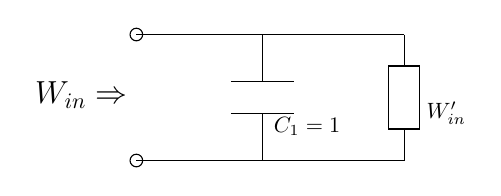
\begin{tikzpicture}[scale=0.8, transform shape]
  % Coordinates
  \coordinate (A) at (-0.02, 1.04);
  \coordinate (L) at (2.71, 0.27);
  \coordinate (B) at (0.00, 2.00);
  \coordinate (C) at (0.00, 0.00);
  \coordinate (D) at (2.00, 0.00);
  \coordinate (E) at (2.00, 2.00);
  \coordinate (F) at (1.50, 1.25);
  \coordinate (G) at (2.50, 1.25);
  \coordinate (H) at (1.50, 0.75);
  \coordinate (I) at (2.50, 0.75);
  \coordinate (J) at (2.00, 0.75);
  \coordinate (K) at (2.00, 1.25);
  \coordinate (M) at (4.25, 0.00);
  \coordinate (N) at (4.25, 2.00);
  \coordinate (O) at (4.25, 0.50);
  \coordinate (P) at (4.25, 1.50);
  \coordinate (Q) at (4.92, 0.45);

  % Drawing
  \node[left, font=\Large] at (A) {$W_{in} \Rightarrow$};
  \node[above] at (L) {$C_1=1$};
  \draw (B) circle (0.10);
  \draw (C) circle (0.10);
  \draw (C) -- (D);
  \draw (B) -- (E);
  \draw (F) -- (G);
  \draw (H) -- (I);
  \draw (D) -- (J);
  \draw (E) -- (K);
  \draw (D) -- (M);
  \draw (E) -- (N);
  \draw (4,0.5) rectangle (4.5,1.5);
  \draw (M) -- (O);
  \draw (N) -- (P);
  \node[above] at (Q) {$W_{in}'$};
\end{tikzpicture}  

$W_{in}(0) = 1 \hat{=}$ Durchlassbereich


$W_{in} = \frac{1}{V_{in}}$\\
Wechsel in Admittanzebene: $V_{in} = sC_1 + V_{in}' \Leftrightarrow V_{in}' = V_{in} -s = \frac{2 s^3 + 2s^2 + 2s + 1 - 2s^3 - 2s^2 - s}{2s^2 + 2s + 1} = \frac{s + 1}{2s^2  + 2s + 1}$

$W_{in}' = \frac{2s^2 + 2s + 1}{s + 1}$

$\lim_{s \rightarrow \infty} W_{in}(s)' = 2s \Rightarrow$  induktiv $L = 2$

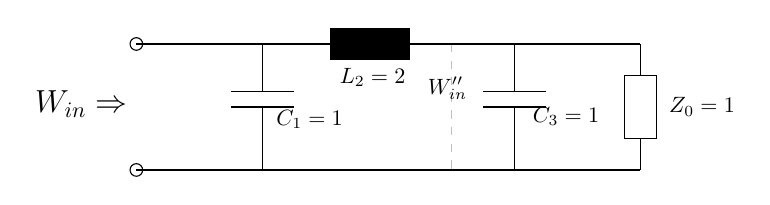
\begin{tikzpicture}[scale=0.8, transform shape]
  % Coordinates
  \coordinate (A) at (-0.02, 1.04);
  \coordinate (L) at (2.75, 0.53);
  \coordinate (B) at (0.00, 2.00);
  \coordinate (C) at (0.00, 0.00);
  \coordinate (D) at (2.00, 0.00);
  \coordinate (E) at (2.00, 2.00);
  \coordinate (F) at (1.50, 1.25);
  \coordinate (G) at (2.50, 1.25);
  \coordinate (H) at (1.50, 1.00);
  \coordinate (I) at (2.50, 1.00);
  \coordinate (J) at (2.00, 1.00);
  \coordinate (K) at (2.00, 1.25);
  \coordinate (M) at (5.00, 0.00);
  \coordinate (N) at (5.00, 2.00);
  \coordinate (O) at (3.75, 1.20);
  \coordinate (P) at (4.94, 0.99);
  \coordinate (Q) at (6.82, 0.58);
  \coordinate (R) at (5.50, 1.25);
  \coordinate (S) at (6.50, 1.25);
  \coordinate (T) at (5.50, 1.00);
  \coordinate (U) at (6.50, 1.00);
  \coordinate (V) at (6.00, 1.00);
  \coordinate (W) at (6.00, 1.25);
  \coordinate (X) at (6.00, 0.00);
  \coordinate (Y) at (6.00, 2.00);
  \coordinate (Z) at (8.00, 0.00);
  \coordinate (AA) at (8.00, 2.00);
  \coordinate (AB) at (8.00, 0.50);
  \coordinate (AC) at (8.00, 1.50);
  \coordinate (AD) at (8.98, 0.73);

  % Drawing
  \node[left, font=\Large] at (A) {$W_{in} \Rightarrow$};
  \node[above] at (L) {$C_1=1$};
  \draw (B) circle (0.10);
  \draw (C) circle (0.10);
  \draw (C) -- (D);
  \draw (B) -- (E);
  \draw (F) -- (G);
  \draw (H) -- (I);
  \draw (D) -- (J);
  \draw (E) -- (K);
  \draw (D) -- (M);
  \draw (E) -- (N);
  \draw[fill=black] (3.09,1.75) rectangle (4.34,2.25);
  \node[above] at (O) {$L_2 = 2$};
  \draw[lightgray, dashed] (N) -- (M);
  \node[above] at (P) {$W_{in}''$};
  \node[above] at (Q) {$C_3
=1$};
  \draw (R) -- (S);
  \draw (T) -- (U);
  \draw (X) -- (V);
  \draw (Y) -- (W);
  \draw (M) -- (Z);
  \draw (N) -- (AA);
  \draw (7.75,0.5) rectangle (8.25,1.5);
  \draw (Z) -- (AB);
  \draw (AA) -- (AC);
  \node[above] at (AD) {$Z_0 = 1$};
\end{tikzpicture}

$W_{in}' = sL_2 + W_{in}'' \Rightarrow W_{in}'' = W_{in}' - sL_2 = \frac{2s^2 + 2 + 1 - 2s^2 - 2s}{s + 1} = \frac{1}{s + 1}$

$V_{in}'' = \frac{1}{W_{in}''} = s + 1 \hat{=} $ Parallelschaltung $C_3 = 1$ und $Z_0 = 1$


Wahl des positiven VZ: 
$W_{in} = \frac{s^3 + 2s^2 + 2s + 1 + s^3}{s^3 + 2s^2 + 2s + 1 - s^3} = \frac{2s^3 + 2s^2 + 2s + 1}{2s^2 + 2s + 1}$
Noch immer TF, da $W_{in}(0) = 0$


\begin{pitemize}
    \item $\lim_{s\rightarrow\infty} W_{in} = s \Rightarrow$ induktiv $L_1 = 1$
    \item $W_{in} = sL_1 + W_{in}' \Rightarrow W_{in}' = \frac{2s^3 + 2s^2 + 2s + 1 - 2s^3 - 2s^2 - s}{2s^2 + 2s + 1} = \frac{s + 1}{2s^2 + 2s + 1}$
    \item $\lim_{s\rightarrow\infty} W_{in}' = \frac{1}{2s} \Rightarrow$ kapazitiv $C_2 = 2$
    \item $V_{in}' = sC_2 + V_{in}'' \Rightarrow V_{in}'' = \frac{2s^2 + 2s + 1 - 2s^2 - 2s}{s + 1}$
\end{pitemize}



\subsection{LC-Hochpassfilter mit Butterworthverhalten}

vom TP: $\abs{S_{21}}^2 = \frac{1}{1 + \left(\frac{s}{s_C}^{2m}\right)}$
Übergang zum HP durch subsitution $s->\frac{1}{s}$
HP: $\abs{S_{21}}^2 = \frac{1}{1 + \left(\frac{s_C}{s}^{2m}\right)}$

\subsubsection{Beispiel}

$m = 3$, $s_c = j $

$\abs{S_{21}}^2 = \frac{1}{1 + \frac{-1}{s^6}} = \frac{s^6}{s^6 - 1}$

$\abs{S_{11}}^2 = 1 - \abs{S_{21}}^2 = \frac{-1}{s^6 -1} = \frac{1}{1 - s^6} = S_{11}(s) S_{11}(-s)$
$S_{11}(s) = \frac{\pm 1}{s^3 + 2s^2 + 2s + 1}$

Wahl des pos. VZ $W_{in} = \frac{1 + S_{11}}{1 - S_{11}} = \frac{s^3 + 2s^2 + 2s + 1 + 1}{s^3 + 2s^2 + 2s + 1 - 1} = \frac{s^3 + 2s^2 + 2s + 2}{s^3 + 2s^2 + 2s}$

HP da $\lim_{s\rightarrow\infty} = 1$

\begin{pitemize}
    \item $\lim_{s\rightarrow0}\limits = \frac{2}{2s} = \frac{1}{s} \Rightarrow C = 1$
    \item Kapazität is serielle
    \item $W_{in}' = W_{in} - \frac{1}{s} = \frac{s^3 + 2s^2 + 2s + 2 - s^2 - 2s - 2}{s^3 + 2s^2 + 2s} = \frac{s^3 + s^2}{s^3 + 2s^2 + 2s} = \frac{s^2 + s}{s^2 + 2s + 2}$
    \item $\lim_{s\rightarrow0}\limits W_{in}' = \frac{s}{2} \Rightarrow L = \frac{1}{2}$
    \item Indiktivität ist parallel 
    \item $V_{in}'' = V_{in}' - sL = \frac{s^2 + 2s + 2 - 2s - 2}{s^2 + s} = \frac{1}{1 + s} \Rightarrow$ Reihenschaltung aus $C = 1$ und $Z_0 = 1$ 
\end{pitemize}






\subsection{Filter aus Induktivitäten und Kapazitäten sowie Leitungselementen}
\bildf{z_img_4}

nicht rendudant

\bildf{z_img_5}

rendudant

beschreibenede Funktion für Butterworth

$\left[K_{UE}\right] = \frac{1}{\sqrt{1 - s^2}}\begin{bmatrix}
    1 & sZ_2 \\ \frac{s}{Z_2} & 1
\end{bmatrix}$

$\begin{bmatrix}
    A & B \\ C & D
\end{bmatrix} = \begin{bmatrix}
    1 & sL_1 \\ 0 & 1
\end{bmatrix} \frac{1}{\sqrt{1 - s^2}} \begin{bmatrix}
    1 & sZ_2 \\ \frac{s}{Z_2} & 1
\end{bmatrix}\begin{bmatrix}
    1 & sL_3 \\ 0 & 1
\end{bmatrix}\begin{bmatrix}
    1 & 0 \\ sC_4 & 1
\end{bmatrix}$

$\left(\frac{1}{\sqrt{1 -s^2}}\right)^n P_{m+n}(s)$

n: Anzahl Leitungselementen
m: Anzahl and Indiktivitäten and Kapazitäten



$\abs{S_{21}(s)}^2 = \frac{1}{1 + \abs{\Sigma_{21}(s)}^2}$

$\abs{\Sigma_{21}(s)}^2 = \left(\frac{s^2}{s_c^2}\right)^m \left(\frac{s^2}{s_c^2}\right)^n \frac{\left(1 - s_c^2\right)^n}{\left(1 - s^2\right)^n}$ TP mit Butterworth


geg:: $W_{in}(s)$:

\bildf{z_img_3}
$W_{in} = Z_1 \frac{W_1(s) + sZ_1}{Z_1 + sW_1(s)}$

Auflösen nach $W_1(s)$: 
$W_1(s) = \frac{Z_1 (sZ_1 - W_{in})}{sW_{in} - Z_1}$

$W_{in}(s=1) = Z_1 \frac{W_1(1) + Z_1}{Z_1 + W_1(1)} = Z_1$


Zum Zeitpunkt t=0s => Spannungssprung am Leitungsanfang $\rightarrow t = 0 \rightarrow$ Verhältnis von Spannung zu Strom $\hat{=}$ Leitungswellenwiderstand $Z_1$

Grenzwertsatz der Laplace-Transformation: $f(0+) = \lim_{p\rightarrow\infty} \limits p F(p)$ mit $p = j\omega \Leftrightarrow \omega = -jp$

mit $s = j \tan(\frac{\pi}{2} \frac{\omega}{\omega_0}) = j \tan(\frac{\pi}{2} \left(\frac{-jp}{\omega_0}\right))$

$\lim_{p\rightarrow\infty} \limits j \tan(\frac{\pi}{2} \left(\frac{-jp}{\omega_0}\right)) = 1 \Rightarrow p \rightarrow \infty \hat{=} s \rightarrow 1$

$W_{in}(s) = W_{in}(1) \frac{sW_{in}(1) - W_{in}(s)}{sW_{in}(s) - W_{in}(1)}$

Zähler und Nenner NS bei s = 1 und s= -1s

$(1+s)(1-s) = (1-s^2)$


\subsubsection{Beispiel}

$W_{in}(s) = \frac{1 + 3s + \frac{1}{2}s^2}{1 + \frac{3}{2}s + 2 s^2}$

\begin{penumerate}
    \item Ist ein UE enthalten? $W_{in}(1) \overset{!}{=} - W_{in}(-1)$
    \begin{pitemize}
        \item $W_{in}(1) = \frac{1 + 3 + \frac{1}{2}}{1 + \frac{3}{2} + 2} = 1 = Z_1$
        \item $-W_{in}(1) = -\frac{1 - 3 + \frac{1}{2}}{1 - \frac{3}{2} + 2} = 1$
        \item \bildf{z_img_6}
    \end{pitemize}
    \item Abspaltung
    \begin{pitemize}
        \item $W_{in}'(s) = \frac{s - \frac{1 + 3s + \frac{1}{2}s^2}{1 + \frac{3}{2}s + 2 s^2}}{\frac{1 + 3s + \frac{1}{2}s^2}{1 + \frac{3}{2}s + 2 s^2} - 1} = \frac{s + \frac{3}{2}s^2 + 2s^3 - 1 - 3s - \frac{1}{2}s^2}{s + 3s^2 + \frac{1}{2}s^3 -1-3s -2s^2} = \frac{2s^3 + s^2 - 2s - 1}{\frac{1}{2}s^3 + s^2 - \frac{1}{2}s - 1} = \frac{2s + 1}{\frac{1}{2}s + 1}$
    \end{pitemize}
    \item Ist UE enthalten
    \begin{pitemize}
        \item $W_{in}'(1) = \frac{3}{\frac{3}{2}} = 2 = Z_2$
        \item $-W_{in}+(-1) = -\frac{-1}{\frac{1}{2}} = 2$
        \item \bildf{z_img_7}
    \end{pitemize}
    \item Abspaltung
    \begin{pitemize}
        \item $W_{in}''(s) = 2\frac{s2 - \frac{2s + 1}{\frac{1}{2}s + 1}}{s\frac{2s + 1}{\frac{1}{2}s + 1} - 2} = 2\frac{s^2 + 2s - 2s - 1}{2s^2 + s - s - 2} = \frac{s^2 - 1}{s^2 - 1} = 1$
    \end{pitemize}
\end{penumerate}




\subsection{Beispiel}

$W_{in}(s) = \frac{1 + 3s + \frac{1}{2}s^2}{1 + \frac{1}{2}s}$

\begin{penumerate}
    \item $W_{in}(1) = -W_{in}(-1)$:
    \begin{pitemize}
        \item $W_{in}(1) = \frac{1 + 3 + \frac{1}{2}}{1 + \frac{1}{2}} = 3 = Z_1$
        \item $W_{in}(-1) = \frac{1 - 3 + \frac{1}{2}}{1 - \frac{1}{2}} = -3$
        \item \bildf{z_img_1}
    \end{pitemize}
    \item Abspaltung: $W_{in}'(s) = \frac{3 (3s - \frac{1 + 3s + \frac{1}{2}s^2}{1 + \frac{1}{2}s})}{s\frac{1 + 3s + \frac{1}{2}s^2}{1 + \frac{1}{2}s} - 3} = 3\frac{3s + \frac{3}{2}s^2 - 1 - 3s - \frac{1}{2}s^2}{s + 3 s^2 + \frac{1}{2}s^3 - 3 - \frac{3}{2}s} = 3\frac{s^2 - 1}{\frac{1}{2}s^3 + 3s^2 - \frac{1}{2}s - 3} = \frac{3}{2}\frac{s^2 - 1}{s^3 + 6s^2 - s - 6} = \frac{3}{2} \frac{s^2 -1}{(s^2 - 1)(s + 6)} = \frac{3}{2} \frac{1}{s + 6}$
    \item $V_1(s)' = \frac{1}{6}s + 1$ : Parallelschaltung aus $C$ und $Z_0$ 
\end{penumerate}


\subsubsection{Beispiel}

\bildf{z_img_2}

$W_{in} = s \frac{\frac{1}{s} s}{\frac{1}{s} + s}$

Überprüfung mit Realisierung
\section{Mischer}
\renewcommand{\ort}{topics/Mischer}

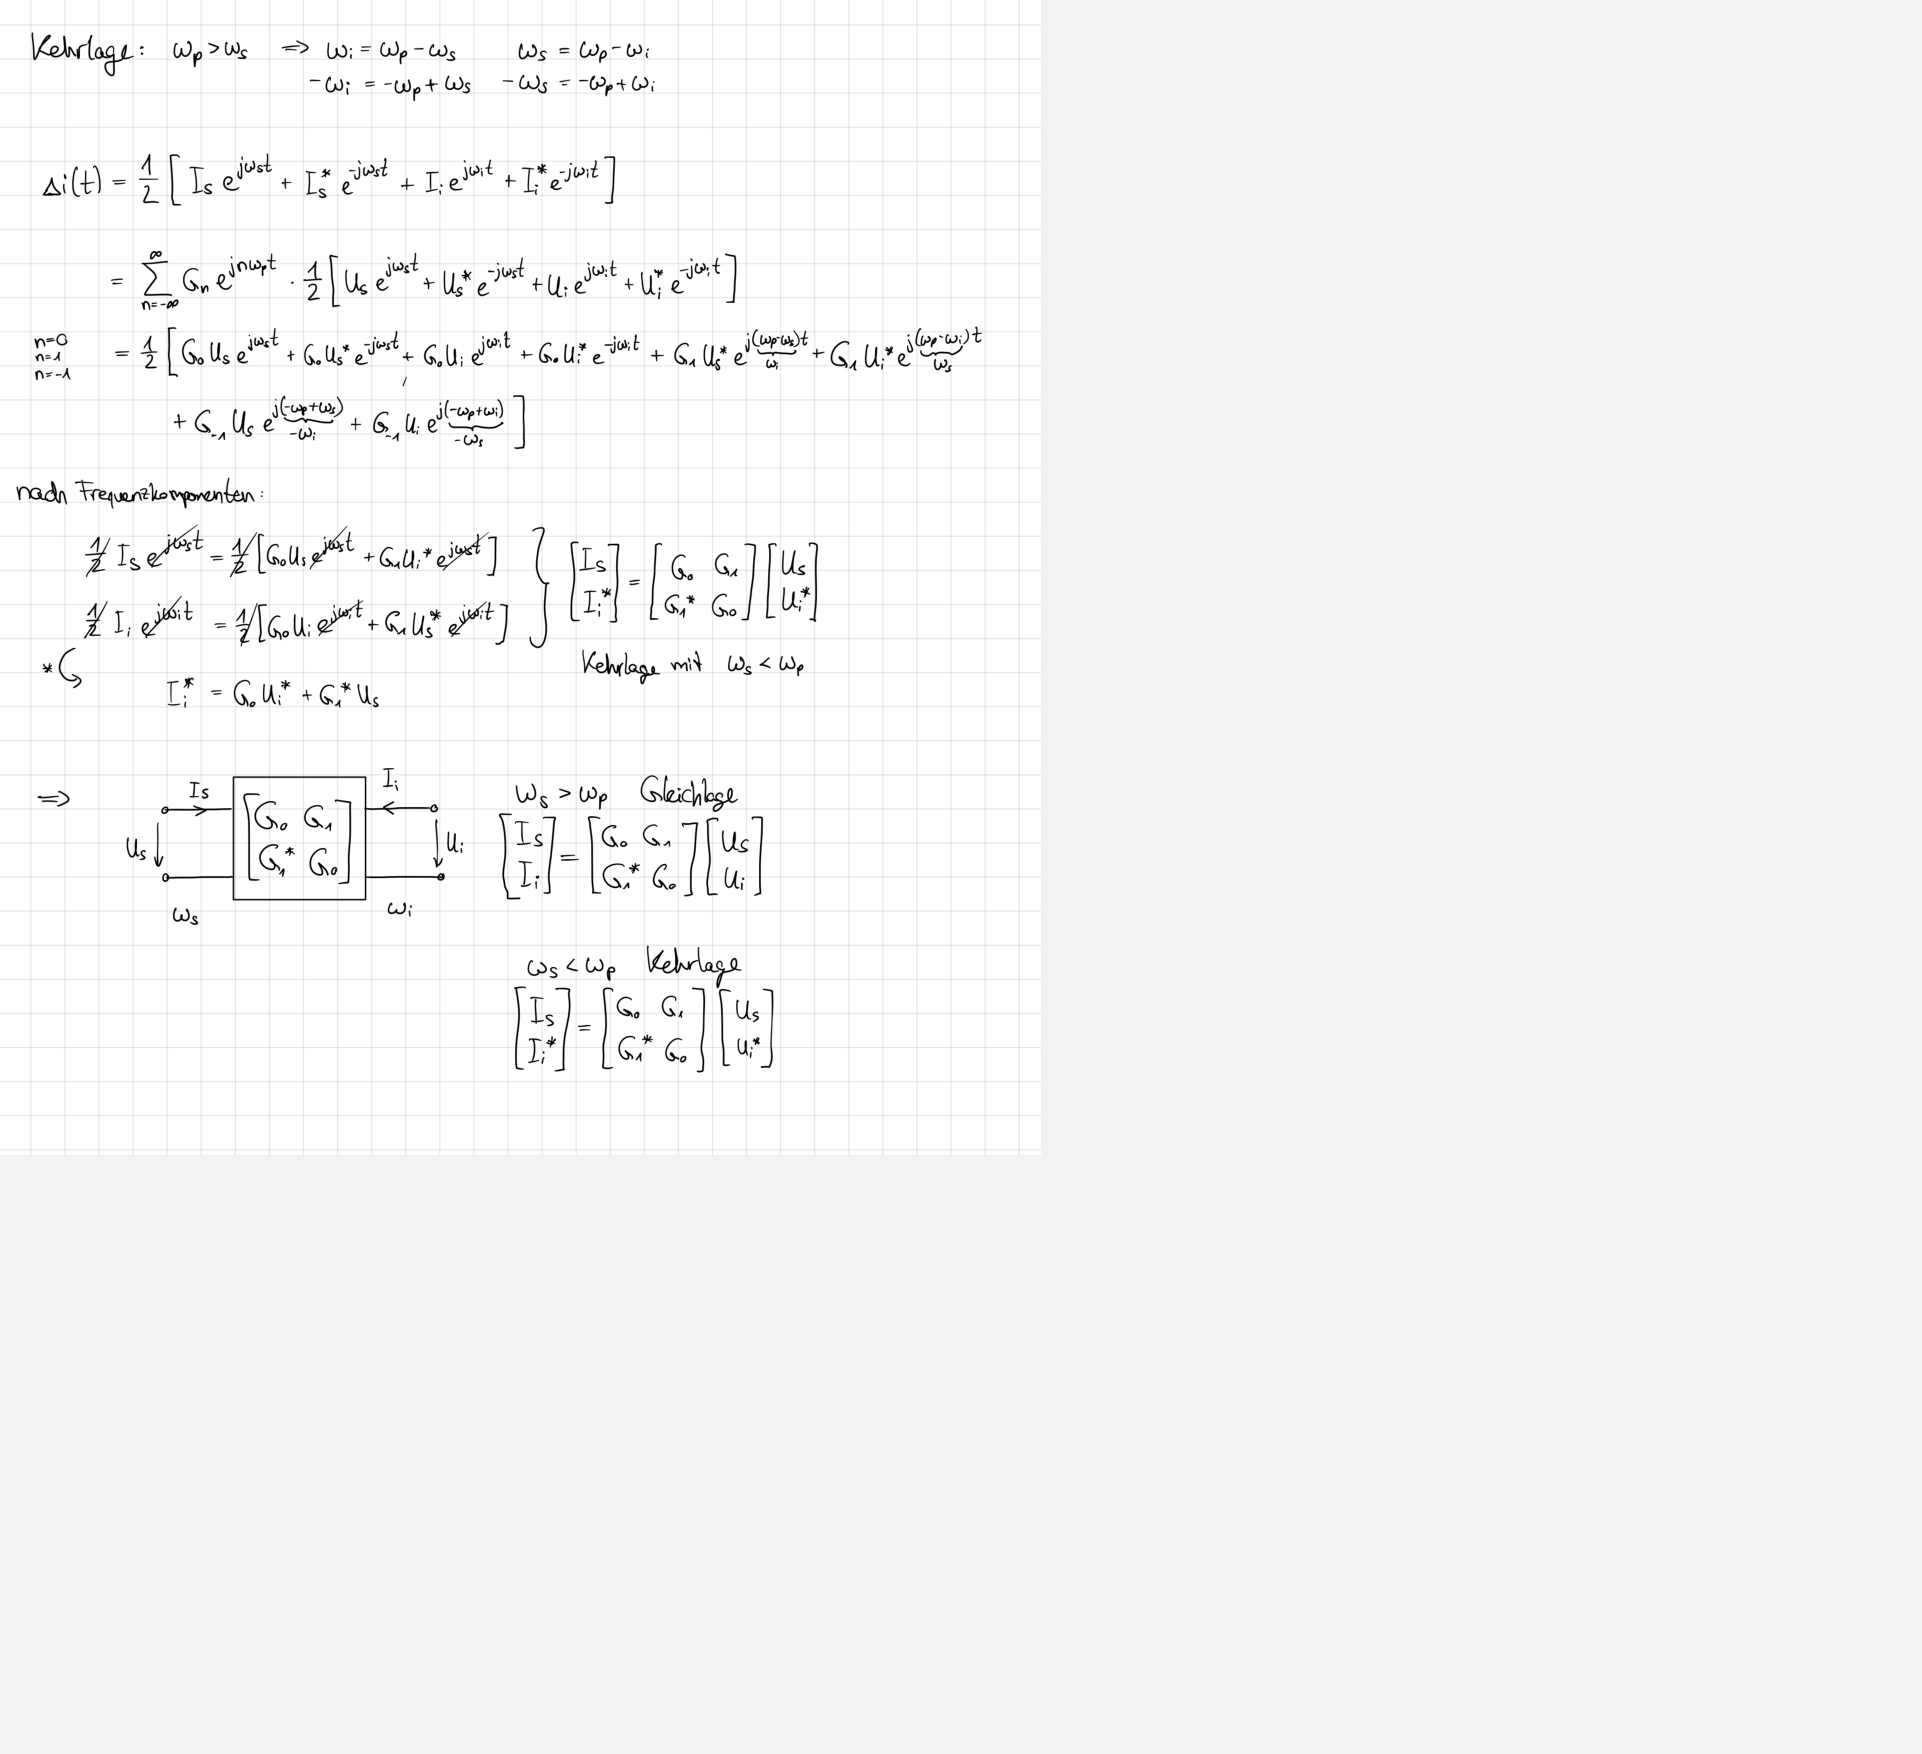
\includegraphics[width=\linewidth,page=1]{topics/Mischer/6. Mischer.pdf}
\includegraphics[width=\linewidth,page=2]{topics/Mischer/6. Mischer.pdf}

\subsection{Breitband-Mischer}

\bildf{BreitbandMischer}

\bildf{ESB BB Mischer}
$\begin{bmatrix}
    I_s \\ I_i \\ I^*_{sp}
\end{bmatrix} = \begin{bmatrix}
    G_0 & G_1 & G_2 \\ G_1^* & G_0 & G_1 \\ G_2^* & G_1^* & G_0 \\
\end{bmatrix} \begin{bmatrix}
    U_2 \\ U_i \\ U_sp^*
\end{bmatrix}$


\bildf{ESB Mischer}

$\begin{bmatrix}
    I_s \\ I_i
\end{bmatrix} = \begin{bmatrix}
    G_0 & G_1 \\ G_1^* & G_0
\end{bmatrix}\begin{bmatrix}
    U_s \\ U_i
\end{bmatrix}$


$I_sg = I_s + Y_s U_s$


$I_i = -Y_i U_i$

$\begin{bmatrix}
    I_{sg} \\ 0
\end{bmatrix} = \begin{bmatrix}
    G_0 + Y_s & G_1 \\ G_1^* & G_0 + Y_i
\end{bmatrix}\begin{bmatrix}
    U_s \\ U_i
\end{bmatrix}$

Gewinn $G_P = \frac{\text{Ausgangsleistung}}{\text{verfügbare Generatorleistung}}$

\bildf{verf Pgen}

$P_{g,av} = \frac{1}{2} \Re \{U_s I_s^*\}$

$U_s = \frac{I_{sg}}{Y_s + Y_s^*}$

$I_s = I_{sg} \frac{Y_s^*}{Y_s + Y_s^*}$

$\Rightarrow P_{g,av} = \frac{1}{2} \Re \left\{ \frac{I_{sg}I_{sg}^*Y_s}{(Y_s + Y_s^*)(Y_s + Y_s^*)^*}\right\}
= \frac{\abs{I_{sg}}^2}{8\Re \{Y_s\}}$

Ausgangsleistung: $P_2 = \frac{1}{2} \Re \{U_iI_i^*\} = \frac{1}{2} \Re \{U_iU_i^*Y_i\} = \frac{1}{2} \abs{U_i}^2 \Re\{Y_i\}$


$G_P = \frac{\frac{1}{2}\abs{U_i}^2 \Re\{Y_i\}}{\frac{1}{8}\abs{I_{sg}}^2 \frac{1}{\Re \{Y_s\}}}
= 4\abs{\frac{U_i}{I_sg}}^2 \Re\{Y_i\}\Re\{Y_s\}$


$\begin{bmatrix}
    U_s \\ U_i \end{bmatrix}= \begin{bmatrix}
        \tilde{G}
    \end{bmatrix}^{-1} \begin{bmatrix}
        I_{sg} \\ 0
    \end{bmatrix} = \frac{1}{(G_0 + Y_s)(G_0 + Y_i) - \abs{G_1}^2} \begin{bmatrix}
        G_0 + Y_i & -G_1 \\ -G_1^* & G_0 + Y_s
    \end{bmatrix} \begin{bmatrix}
        I_{sg} \\ 0
    \end{bmatrix}
$
$\frac{U_i}{I_{sg}} = \frac{-G_1^*}{(G_0 + Y_s)(G_0 + Y_i) - \abs{G_1}^2}$


$\Rightarrow G_P = 4 \frac{\abs{G_1}^2\Re\{Y_i\}\Re\{Y_s\}}{\abs{(G_0 + Y_s)(G_0 + Y_i) - \abs{G_1}^2}^2}$


\subsection{Ausführungsformen von Mischern}

\subsubsection{Ein Dioden Mischer}
\bildf{1DiodenMischer}

Elemente zu Verfügung
\begin{pitemize}
    \item \bildfR{0.1}{zimg1}
    \item \bildfR{0.1}{zimg2}
    \item \bildfR{0.1}{zimg4}
    \item \bildfR{0.1}{zimg3}
\end{pitemize}

\bildf{DiodeKS}


\subsubsection{Zwei Dioden Mischer}


\bildf{2DiodenMischer}


$u_p(t) = \hat{u}_p \cos(\omega_p t)$

$u_s(t) = \hat{u}_s \cos(\omega_s t + \varphi_s)$

Diode 1: $u_{D1}(t) \frac{1}{\sqrt{2}} \hat{u}_p \cos(\omega_p t) + \frac{1}{\sqrt{2}} \hat{u}_s \cos(\omega_s t + \varphi_s + 90^\circ)$

Diode 2: $u_{D2}(t) \frac{1}{\sqrt{2}} \hat{u}_p \cos(\omega_p t + 90^\circ) + \frac{1}{\sqrt{2}} \hat{u}_s \cos(\omega_s t + \varphi_s)$

$\Rightarrow u_i(t) = \kappa G_1 \hat{u}_s \cos\left((\omega_s - \omega_p)t + \varphi_s  90^\circ\right)$

$u_i(t) = \kappa G_1 \hat{u}_s \cos\left( \omega_i t + \varphi_s + 90^\circ\right)$


Einfach balancierter Mischer
Rauschbalancierung $\Rightarrow$ Amplitudenschwankungen eben sich auf durch guten Gleichlauf der Dioden.
und ihre entgegengesetzt orientierte Einbaurichtung.

\subsubsection{4-Dioden-Mischer}


\bildf{4DiodenMischer}

ZF$-$Phase resultiert als Differenzphase hier all ZF$-$Pfeile.
Parallel $Rightarrow$ summieren sich auf.
\begin{pitemize}
    \item Rauschbalancierung $\rightarrow$ Amplitudenschwankungen heben sich auf.
    \item Signalbalancierung: RF$-$LO, RF$-$ZF, LO$-$ZF, da alle Tore entkoppelt sind.
\end{pitemize}


Für höherfrequente Realisierung $\Rightarrow$ Einsatz von Kopplern

\bildf{4DiodenMischer mit RK}


Phasenregelkreise
\begin{pitemize}
    \item Synthesegenerator
    \item Stabilisierung von Signalen
\end{pitemize}



Skalar Netzwerkanalysator

\bildf{skalarNWA}

Vektorielle Netzwerkanalysatoren

\bildf{vektorNWA}


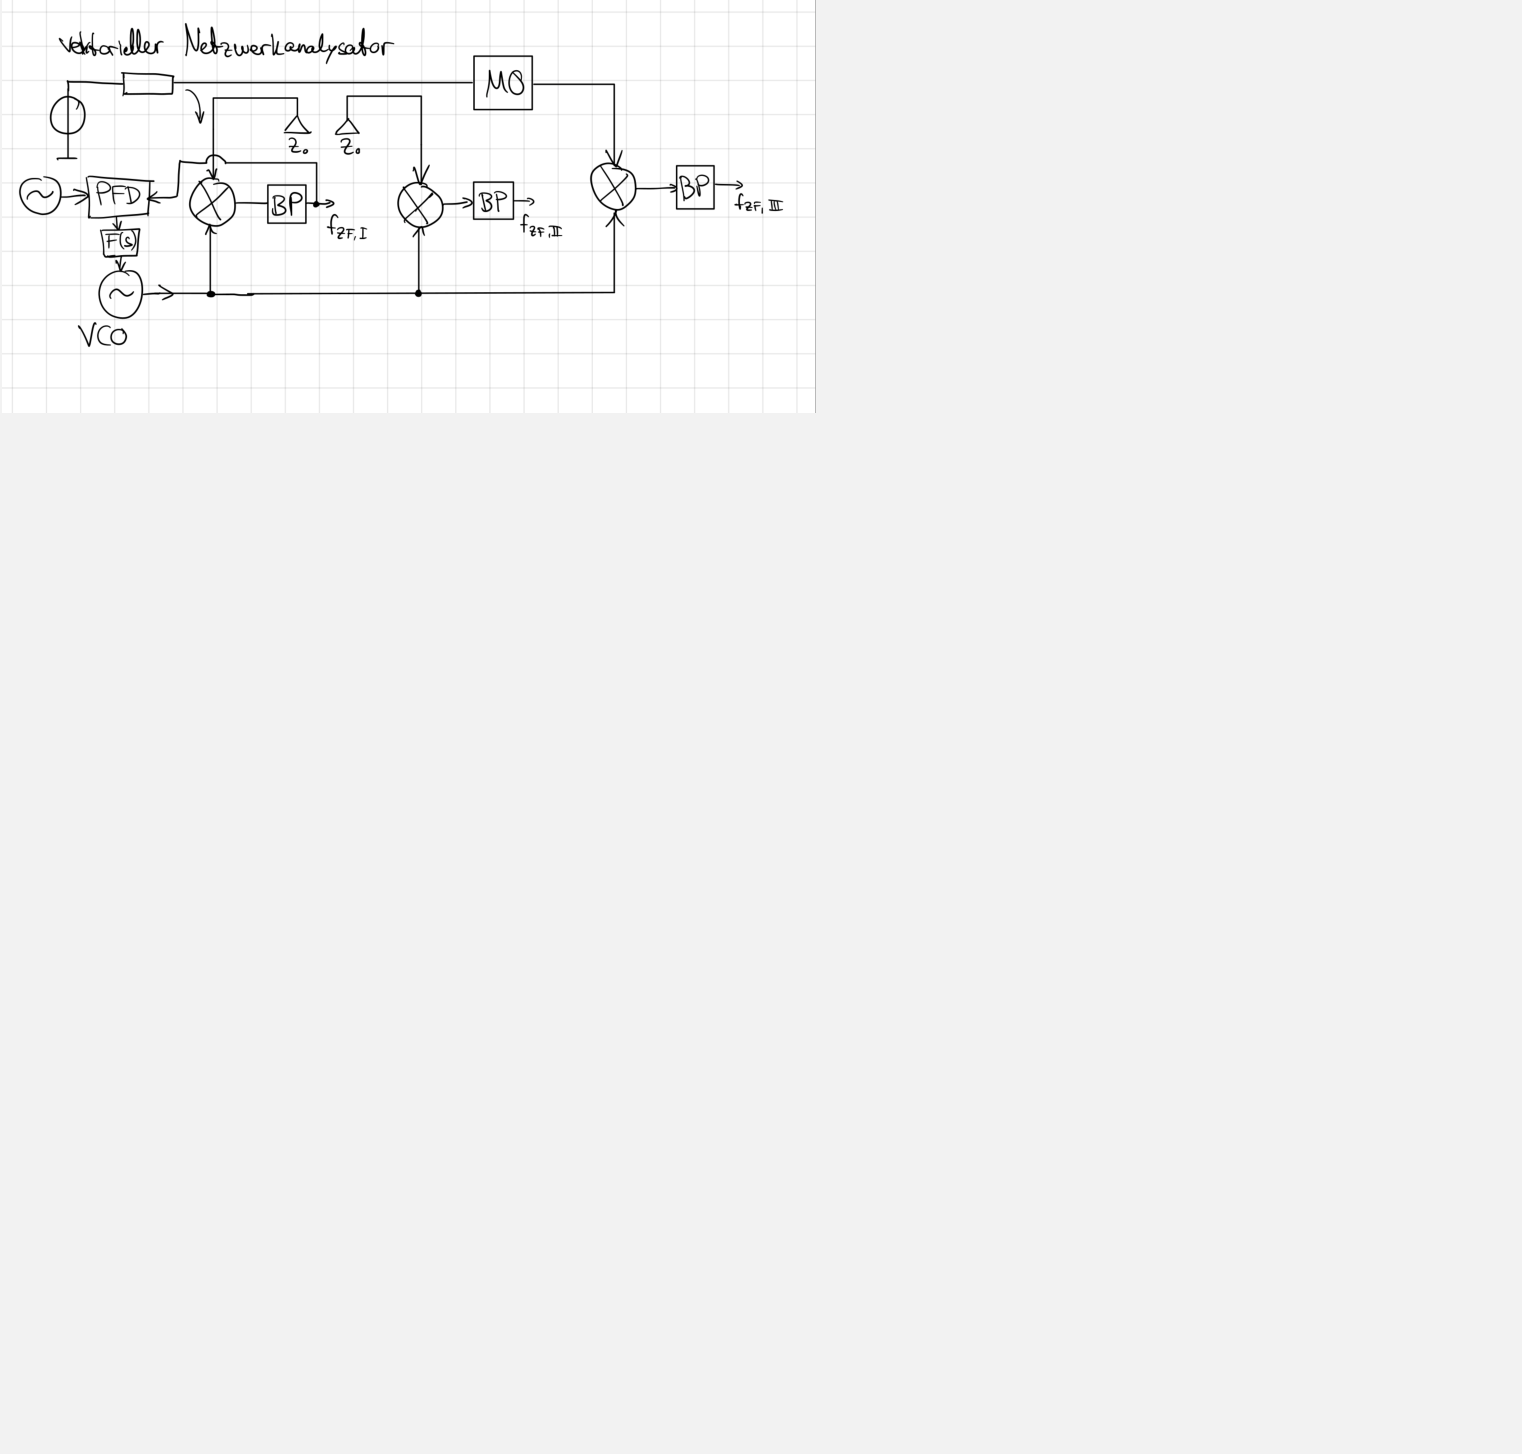
\includegraphics[width=\linewidth,page=1]{topics/Mischer/7.Phasenregelkreise.pdf}
\includegraphics[width=\linewidth,page=2]{topics/Mischer/7.Phasenregelkreise.pdf}
\includegraphics[width=\linewidth,page=3]{topics/Mischer/7.Phasenregelkreise.pdf}
\includegraphics[width=\linewidth,page=4]{topics/Mischer/7.Phasenregelkreise.pdf}




\subsection{Digitale Phasendiskriminatoren}

\subsubsection{Exklusiv Oder- Gatter}

$I_R^V$ Xor Y

\begin{tabular}{cc|c}
    R & V & Y\\
    0 & 0 & 0\\
    0 & 1 & 1\\
    1 & 0 & 1\\
    1 & 1 & 0
\end{tabular}

Vor.: Tastverhältnis der Signale 50\%

\fb \\

$\theta_e = \theta_R - \theta_V$

stabiler Regelpunkt bei $90^\circ$: 
\begin{itemize}
    \item Nicht seitenbandselektiv.
    \item Recktecksingale mit 50\% Tastverhältnis
\end{itemize}


\subsubsection{Flip Flop als unsymmetris. PD}

\fb \\

S = Set 
R = Reset 

\fb FF\\

\fb Die 9 Plots. \\ 

\fb Plot von Uq und Theta e\\

\begin{itemize}
    \item seitenbandselektiv
    \item flankengesteuert
\end{itemize}


\subsection{Phasen-Frequenz-Diskriminatoren PFD}

\fb Shaltbild\\

Zustandgraph:\\

\begin{pitemize}
    \item $\uparrow 0 \hat{=}$ Flanke am Ref. Eingang.
    \item $0 \uparrow \hat{=}$ Flanke am VCO Eingang.
    \item $00 \hat{=}$ Keine Flanke.
    \item $\uparrow \uparrow \hat{=}$ Flanke am Ref. und VCO Eingang.
\end{pitemize}

$U_q = A-B$

3 Zustände $\Rightarrow$ frequenzselektiv
$K_d = \frac{U_h}{2 \pi}$


\subsection{Schritt-/Synthesegeneratoren}
\fb \\

\begin{pitemize}
    \item Reproduzierbare Frequenzeinstellung
    \item Kleine Einschwingzeit für schnelle Einstellung
    \item Kleines $\Delta f$ für lineare Rampe
    \item Optimales Phasenrauschen
\end{pitemize}


\subsubsection{Einschleifiger Phasenregelkreis}
Realisierung eines Schrittgenerators

\fb \\

\begin{pitemize}
    \item $\Delta f = f_{Ref}$
    \subitem $\Delta f \downarrow \rightarrow f_{Ref} \downarrow \rightarrow N \uparrow$
    \item Phasenrauschen des VCO
    \subitem $W_V \sim N^2$
    \item Eckfrequenz des Regelkreises $F(s)$
    \subitem $f_c \approx \frac{1}{20} f_{Ref}$
    \subitem $f_{Ref} \downarrow \rightarrow f_c \downarrow \rightarrow$ Langsames Einschwingungsverhalten
\end{pitemize}


\subsubsection{PLL mit Mischer}

\fb \\

\begin{pitemize}
    \item $f_V = f_{Lo} \pm N f_{Ref}$
    \item $\Delta f_V = f_{Ref}$
    \item Kleinere Teilungsfaktor $\rightarrow$ geringeres Phasenrauschen
    \item keine Reduktion der Frequenzschrittweite
\end{pitemize}

\subsubsection{Verschachtelte PLL}

\fb \\


\begin{pitemize}
    \item $f_z = \abs{f_v - f_{v2}}$
    \item $f_{v2} = L f_{Ref}$
    \item $f_{v3} = N f_{Ref}$
    \item $f_{v3} = M f_{z} $
    \item $f_v = f_{v2} \pm f_z = L \cdot f_{Ref} \pm \frac{N \cdot f_{Ref}}{M}$
    \item $\Delta f_v = \frac{f_{Ref}}{M}$
\end{pitemize}


\subsection{PLL mit fraktionalem Teiler}

\fb Schaltbild\\

\fb N über Zeit\\

\begin{pitemize}
    \item M Takte einer Periode T
    \item Zeitl. Mittelwert: $\bar{N} = \frac{(M - k)N + k(N + 1)}{M} = N + \frac{k}{M}$
    \item $f_v = (N + \frac{k}{M}) f_{Ref}$
\end{pitemize}          

Frequenzrampe
\fb Frequenzrampe \\

wirkt wie zufälliges "Umschalten" des Teilungsfaktor $\rightarrow$ noise shaping $\rightarrow$ um Störsignale zu unterdrücken, die bei periodischen umschalten erscheinen.

\fb Spektrum \\

\fb Frequenzrampe \\

\begin{pitemize}
    \item N wird im gleichen Zeitabständen $\Delta T$ verändert
    \item Bandbreite $B = f_{max} - f_{min} = N_{max} f_{Ref} - N_{min} f_{Ref} = Zf_{Ref} $
    \item Rampendauer: $T = Z \Delta T = Z \frac{1}{f_{Ref}}$
    \item $BT = Z^2 \Leftrightarrow Z = \sqrt{BT}$
\end{pitemize}




\section{VNA}
\renewcommand{\ort}{topics/VNA}


\subsection{skalares NWA}

\fb NWA\\


\begin{pitemize}
    \item $\abs{S_{21}}^2 ,\abs{S_{11}}^2$ können aus Leistungsmessungen
    \item durch Umdrehen des MO
    \item nur Fehlerabschätzung
\end{pitemize}

VNA

\fb VNA\\


\fb \\

\begin{pitemize}
    \item Amplituden und Phasen in (was hier) und durch Mischung gewonnen.
    \item Betrag und Phase von $S_{21}, S_{11}$
    \item Durch umdrehen von MO $S_{12}, S_{22}$
    \item Systemfehler
    \begin{pitemize}
        \item Verlust der Zuleitungen und der Systemkomponenten
        \item Fehleranpassung an Steckern, Kabel, Leitungskoppler, Generator
        \item Nichtidealitäten der Mischer und Verstärker
    \end{pitemize} 
\end{pitemize}



\subsection{Linear Fehlermodell}

\fb \\

$\begin{bmatrix}
    b_1 \\ b_2 \\b_3 \\ b_4
\end{bmatrix} = 
\begin{bmatrix}
    K_{11} & K_{12} & K_{13} & K_{14} \\
    K_{21} & K_{22} & K_{23} & K_{24} \\
    K_{31} & K_{32} & K_{33} & K_{34} \\
    K_{41} & K_{42} & K_{43} & K_{44} \\
\end{bmatrix} \begin{bmatrix}
    a_1 \\ a_2 \\ a_3 \\ a_4
\end{bmatrix}$

\begin{pitemize}
    \item $a_2 = r_2 b_2$
    \item $a_4 = r_4 b_4$
\end{pitemize}

\begin{pitemize}
    \item $b_1 = K_{11} a_1 + K_{12} r_2 b_2 + K_{13} a_3 + K_{14} r_4b_4$
\end{pitemize}
Es gelingt, $a_1$ und $b_1$ zu eliminieren durch Umformen und Einsetzen.
Zusammenhang zwischen $b_2, b_4, a_3, b_3$
Viertor-Zweitor-Reduktion

\begin{pitemize}
    \item $m_f = \nu_2 b_2$
    \item $m_r = \nu_4 b_4$
    \item $\nu_2,\nu_4 = $ f(Mischerkonversionsfaktors, ZF-Verstärkung) 
    \item $R_{11} f(K_{11}, ..., r_2, r_4, \nu_2, \nu_4)$
\end{pitemize}

\fb R block\\

\begin{pitemize}
    \item $m_r = R_{11}m_f + R_{12} a_3$
    \item $b_3 = R_{21} m_f + R_{22} a_3$
\end{pitemize}



\subsubsection{Nach Viertor-Zweitor-Reducktion}

\fb \\

\begin{pitemize}
    \item bestimmbar/bekannt aus Messungen:
    \subitem $m_r, m_f, m_t$
    \item unbekannt: $[R], [T]$
    \subitem Bestimmung aus Kalibrierung
    \item Kalibrierung:Ersetzen des MO durch bekannte Reflektionstandards.
    \begin{pitemize}
            \item $m_r = R_{11}m_f + R_{12}\Gamma b_3$
            \item $b_3 = R_{21}m_f + R_{22} \Gamma b_3$
            \item $b_3 = \frac{R_{21}m_f}{1 - R_{22}\Gamma}$
            \item $\mu = \frac{m_r}{m_f} = R_{11} + \frac{R_{12}R_{21}\Gamma}{1 - R_{22}\Gamma}$
        \end{pitemize}
    \begin{penumerate}
        \item Anpassung: $\Gamma = 0 \Rightarrow \mu_1 = \frac{m_{r1}}{m_{f1}} = R_{11}$
        \item KS: $\Gamma = -1 \Rightarrow \mu_2 = \frac{m_{r2}}{m_{f2}} = R_{11} - \frac{R_{12}R_{21}}{1 + R_{22}}$
        \item LL: $\Gamma = 1 \Rightarrow \mu_3 = \frac{m_{r3}}{m_{f3}} = R_{11}+ \frac{R_{12}R_{21}}{1 - R_{22}}$
    \end{penumerate} 
\end{pitemize}



\end{document}